% Auriga theme
% https://github.com/anishathalye/auriga

\documentclass[14pt,aspectratio=169]{beamer}
\usepackage{pgfpages}
\usepackage{fancyvrb}
\usepackage{tikz}
\usepackage{pgfplots}

\ifnotes
\setbeamertemplate{note page}[plain]
\setbeameroption{show notes on second screen=right}
\fi

\usetheme{auriga}
\usecolortheme{auriga}

% define some colors for a consistent theme across slides
\definecolor{red}{RGB}{181, 23, 0}
\definecolor{blue}{RGB}{0, 118, 186}
\definecolor{gray}{RGB}{146, 146, 146}

\title{\normalsize{Estrategias para la exploración coordinada multi-VANT}}

\author{Luis Alberto Ballado Aradias \\\vspace{0.5cm}
  \and Dr. José Gabriel Ramírez Torres \\
  \and Dr. Eduardo Arturo Rodríguez Tello}

\institute[shortinst]{CINVESTAV - UNIDAD TAMAULIPAS}

\begin{document}

{
  % rather than use the frame options [noframenumbering,plain], we make the
  % color match, so that the indicated page numbers match PDF page numbers
  \setbeamercolor{page number in head/foot}{fg=background canvas.bg}
  \begin{frame}
    \titlepage
  \end{frame}
}

\begin{frame}{\color{blue}Antecedentes22xsxsxs}

  \note{
    Hablar de los antecedentes en robotica,
    evolucion a robotica de servicios
  }
  
  \begin{itemize}
    \item A \alert{highlighted} bulleted item
      \pause
    \item Another item
      \begin{itemize}
        \item With sub-bullets
        \item And another, with some \textbf{bold} text
      \end{itemize}
    \item And another, at the top level, with \textit{italic} text
  \end{itemize}
  
\end{frame}
%antecedentes
\begin{frame}{\color{blue}Motivaciones}
  
  \note{
    https://ccc.inaoep.mx/~emorales/Papers/2009/eduardo.pdf
    Hablar de la importancia de construir software para robots
  }

  \begin{columns}
    \begin{column}{0.5\linewidth}
      \begin{itemize}
        \item This side has a bullet
        \item And another bullet, with text that wraps if it's long
      \end{itemize}
    \end{column}
    \begin{column}{0.5\linewidth}
      \begin{figure}
        \centering
        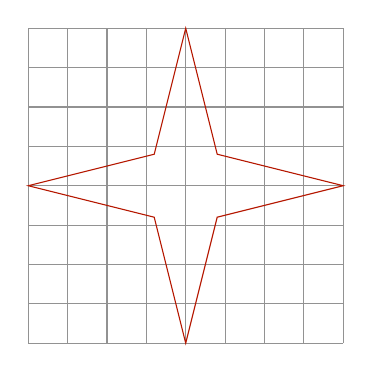
\begin{tikzpicture}[scale=2]
          \draw[step=0.25cm,color=gray] (-1,-1) grid (1,1);
          \draw[color=red] (1,0) -- (0.2,0.2) -- (0,1) -- (-0.2,0.2) -- (-1,0)
          -- (-0.2,-0.2) -- (0,-1) -- (0.2,-0.2) -- cycle;
        \end{tikzpicture}
        \caption{A figure caption}
      \end{figure}
    \end{column}
  \end{columns}

  \note{
    This slide has notes too.
  }

\end{frame}
%motivaciones
\begin{frame}{\color{blue}Planteamiento del problema}
  
  \begin{figure}
    \centering
    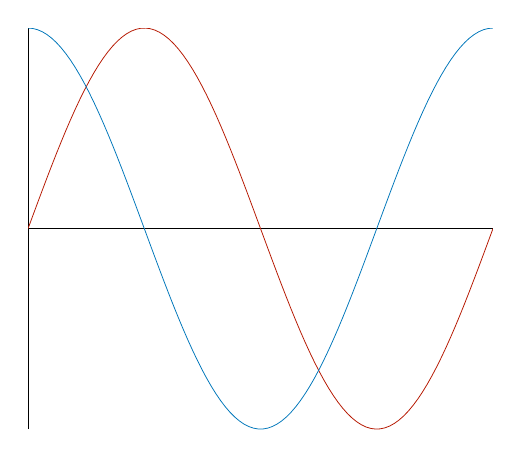
\begin{tikzpicture}[scale=0.7]
      \begin{axis}[
          scale only axis,
          no markers,
          domain=0:2*pi,
          samples=100,
          axis lines=center,
          axis line style={-},
          ticks=none]
        \addplot[red] {sin(deg(x))};
        \addplot[blue] {cos(deg(x))};
      \end{axis}
    \end{tikzpicture}
    \caption{The figure's caption}
  \end{figure}
\end{frame}
%planteamiento problema
\begin{frame}{\color{blue}Hipótesis}
  
  \begin{center}
    Poner la hipótesis acá
  \end{center}

  \vspace{2ex}
  \begin{center}
    \scriptsize (a small note)
  \end{center}

\end{frame}
%hipotesis
\begin{frame}{\color{blue}Preguntas de investigación}

  \begin{itemize}
  \item Pregunta 1\\  %{\color{gray} [Some citation]}
  \item Pregunta 2\\  %{\color{gray} [Another citation]}
  \item Pregunta 3\\  %{\color{gray} [Another citation]}
  \end{itemize}

  %\begin{columns}
  %  \begin{column}{0.5\linewidth}
  %    \footnotesize
  %    Hola mundo
  %  \end{column}
  %  \begin{column}{0.5\linewidth}
  %    {\color{red} Some explanatory text, in red, with some \texttt{monospace} text.}
  %    There might be some math, too:   
  %    $$\sqrt{x} + 2x$$
  %  \end{column}
  %\end{columns}

\end{frame}
%preguntas investigacion
\begin{frame}{\color{blue}Objetivos generales \& particulares}
  
  \begin{itemize}
  \item Some statement {\color{gray} [Some citation]}
  \item Another statement {\color{gray} [Another citation]}
  \item A final statement {\color{gray} [The last citation]}
  \end{itemize}
  
  \vspace{3ex}
  \begin{center}
    \scriptsize (a small note)
  \end{center}
  
\end{frame}

%objetivos generales y particulares
\begin{frame}{\color{blue}Enfoque propuesto}

  %bartolomei
  %https://www.research-collection.ethz.ch/bitstream/handle/20.500.11850/620637/bartolomei_ral2023.pdf?sequence=1&isAllowed=y

  %racer
  %https://ieeexplore.ieee.org/stamp/stamp.jsp?tp=&arnumber=10038280
  
  %Enfoque propuesto

  % proveer la justificación de los metodos utilizados
  % marco experimental
  % La forma de cómo se evaluará el enfoque propuesto
  % Contra que técnicas/metodologias se compararán los resultados
  
  \begin{itemize}
  \item This slide has some text along with a link
    \begin{itemize}
    \item \textbf{Some bold text}: followed by an explanation
    \item \textbf{More bold text}: followed by more text
    \end{itemize}
  \item Another bullet, with sub-bullets
    \begin{itemize}
    \item A sub-bullet
    \item Another sub-bullet, with more text
    \end{itemize}
  \end{itemize}
  
  \vspace{2ex}
  \begin{center}
    \color{blue} \href{https://github.com/anishathalye/auriga}{github.com/anishathalye/auriga}
  \end{center}
  
\end{frame}
%enfoque propuesto

\end{document}
